

\documentclass[conference]{IEEEtran}

\usepackage[brazil]{babel}
\usepackage[utf8]{inputenc}



\ifCLASSINFOpdf
  \usepackage[pdftex]{graphicx}
  \graphicspath{{../pdf/}{../images/}}
  \DeclareGraphicsExtensions{.pdf,.jpeg,.png}
\else
  \graphicspath{{../pdf/}{../images/}}
  \DeclareGraphicsExtensions{.pdf,.jpeg,.png}
\fi


\usepackage{amsmath}
\interdisplaylinepenalty=2500


\usepackage{array}

\ifCLASSOPTIONcompsoc
  \usepackage[caption=false,font=normalsize,labelfont=sf,textfont=sf]{subfig}
\else
  \usepackage[caption=false,font=footnotesize]{subfig}
\fi




\hyphenation{op-tical net-works semi-conduc-tor}


\begin{document}

\title{Trabalho de Inteligência Computacional}

\author{
\IEEEauthorblockN{Diego de Oliveira}
\IEEEauthorblockA{Escola de Artes, Ciências e Humanidades (EACH)\\
Universidade de São Paulo (USP)\\
Email: diego@diegooliveira.com}
}


% make the title area
\maketitle

\begin{abstract}
Iremos demonstrar o uso de algoritmos genéticos na resolução de uma série de funções matemáticas, apresentando os resultados comparativos de várias parametrizações.
\end{abstract}


\IEEEpeerreviewmaketitle



\section{Introdução}

Esse trabalho tem como objetivo apresentar o uso de algoritmos genéticos(AG) na resolução de uma série de funções matemáticas, exercitando o conteúdo apresentado em sala, complementando quando necessário. Será usado a função de Rastrigin como problema de maximização enquanto o de minimização será feita com funções de alta dimensionalidade - unimodais e multimodais.

No AG serão utilizados os operadores de mutação, seleção e cruzamento, aplicando valores diferentes para as chances de utilização de cada um deles. Iremos avaliar o uso de torneio e roleta para o processo de cruzamento além do uso de elitismo na evolução das gerações dos indivíduos.

A forma escolhida para representação do cromossomo é um fator importante na implementação dos algoritmos genéticos tanto no quesito de performance, temporal e espacial, quanto na capacidade de encontrar o ótimo global. Nas sessões seguintes serão discutidos formas de representação do cromossomo para os problemas tratados, explicando vantagens e desvantagens das possíveis abordagens.

Para elaboração do trabalho foram usados uma série de ferramentas. O código do AG foi desenvolvido em Rust, os gráficos foram gerados com \textit{scritps} R e foram usados alguns \textit{scripts bash} pra executar os testes. Rust é uma linguagem de programação elaborada pela Mozilla Fundation e foi escolhida devido ao conhecido desafio de performance dos AGs.

\section{Operadores Genéticos}

Existe uma grande quantidade de operadores que podem ser aplicados no AG tanto para seleção, cruzamento e mutação. Foram codificados para o trabalho os seguintes operadores:

\subsection{Seleção}

Os operadores de seleção são usados na etapa escolha do par de indivíduos que irão participar da etapa de cruzamento.

\begin{itemize}
  \item \textbf{Torneio} - Simula o processo natural de torneio. Deve ser definido um parâmetro $n$ de amostras que serão escolhidas aleatoriamente para duelarem entre si, os dois mais aptos são selecionados pra cruzamento, os demais são reestabelecidos a população.
  \item \textbf{Roleta} - Processo de seleção que simula um a roleta da sorte onde os indivíduos com maior aptidão possuem maior chance de serem sorteados.
\end{itemize}

\subsection{Cruzamento}

O operador de cruzamento é responsável por mesclar dois indivíduos. Foram implementados os seguintes operadores:

\begin{itemize}
  \item \textbf{Cruzamento de um ponto} - Esse operador de cruzamento cria dos filhos, um com parte dos cromossomos do primeiro pai até um ponto $x$ e o resto com cromossomos do segundo pai, e outro com o no sentido inverso.
  \item \textbf{Cruzamento de dois pontos} - Parecido com o primeiro cruzamento porém são selecionados dois pontos de cruzamento.
\end{itemize}

\subsection{Mutação}

O operador de mutação é responsável por adicionar variabilidade na população de indivíduos. Foram implementados os seguintes operadores:

\begin{itemize}
  \item \textbf{Mutação simples} - Escolhe aleatoriamente um ponto do cromossomo e troca por um valor aleatório.
\end{itemize}


\section{Modelo de Avaliação}

Foram feitas várias execuções para avaliar a parametrização e os operadores aplicados aos problemas abordados nesse trabalho.  Inicialmente os valores de mutação e cruzamento foram escolhidos empiricamente, em seguida foram feitos testes para validar sua estabilidade, ajustando quando necessário.

Durante a avaliação dos parâmetros executamos testes com o valor de mutação, variando de $0$ a $100$, incrementando $5$ por vez. Para cada valor d mutação rodamos o AG cinco vezes para avaliar a estabilidade do valor encontrado. Nas funções de maximização iremos tomar o menor valor da série de cinco, nas de minimização o maior, como o as funções são conhecidas será possível a estabilidade.

Para todos os problemas foi usado como critério de parada o número máximo de iterações. Os valores foram ajustados de acordo com os parâmetros usados no AG, formato do cromossomo e sua estabilidade.

\section{A função Rastrigin}

A função de Rastrigin \ref{eq:rastrigin} foi um problema elaborada especificamente para teste de performance em algoritmos de maximização, seu principal desafio se da por conta do amplo espaço de busca e pela existência de vários mínimos locais como pode ser observado na figura \ref{fig:rastrigin}.

\begin{equation}\label{eq:rastrigin}
f(\mathbf{x}) = A n + \sum_{i=1}^n \left[x_i^2 - A\cos(2 \pi x_i)\right]
\end{equation}

Para o trabalho foi proposto a inversa dessa função, o que irá transformar em um problema de maximização, com parâmetros $n=2$, $A=10$ e $x_i\in[-5,5]$. Para esse conjunto de parâmetros o valor máximo já é conhecido, vale $0$. 

\begin{figure}[!t]
        \centering
        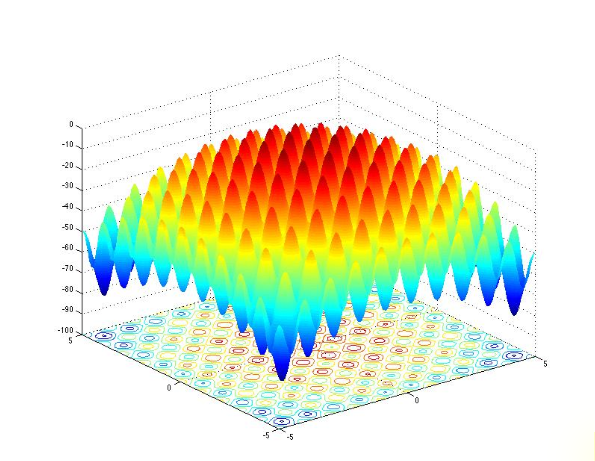
\includegraphics[width=2.5in]{imagens/rastrigin.png}
        \caption{Função Rastrigin para duas variáveis}
        \label{fig:rastrigin}
\end{figure}

\subsection{Modelagem da solução}

Para esse problema foi comparado a performance e precisão da solução ao representar o cromossomo como uma arranjo de pontos flutuantes ou um conjunto de bits.

Ao representar o cromossomo como um arranjo de pontos flutuantes de duas posições, onde a posição zero guarda o valor de $x_1$ e o índice um $x_2$, temos um modelo mais direta e natural ao problema.
 
Na representação como um conjunto de bits será necessário uma codificação que permita representar valores de ponto flutuante. Nos testes foram usados trinta e dois bits para representação de $x$, dezesseis bits para cada $x_i$. A função de transformação para o espaço de busca será feito conforme a equação \ref{eq:rastrigin:cromossomo:bits}, dessa forma o erro será de $0,000015259$.

\begin{equation}\label{eq:rastrigin:cromossomo:bits}
g(x) = -5 + \frac{x}{2^{16}} * 10
\end{equation}

Para seleção do melhor formado do cromossomo e operador de seleção foi feito uma rodada com parâmetros escolhidos empiricamente. A analise dos resultados mostrou que o formato binário tem melhor taxa de convergência para o ponto correto de maximização. Quanto aos algoritmos de seleção, roleta ou torneio, é possível observar que o seletor de torneio se sai melhor. Os melhores resultados estão apresentados na figura \ref{fig:dadosTorneioRastriginBinario}, a figura \ref{dados_rastrigin} apresenta os resultados para outras combinações de formatos e operadores de seleção.

\begin{figure}[h]
        \centering
        \includegraphics[width=2in]{pdf/dados_torneio_rastrigin_binario_elitismo.pdf}%
        \caption{Distribuição do \textit{fitness} nas gerações. A linha azul mostra o maior \textit{fitness}, o vermelho o menor, a amarela o médio e o preto o desvio padrão}
        \label{fig:dadosTorneioRastriginBinario}
\end{figure}

\subsection{Estabilidade dos parâmetros}

As figuras \ref{fig:rastrigin:mut_cross} e \ref{fig:rastrigin:mut_cross_elit} mostram o resultado da série de cinco execuções nas variações do valor de mutação. Como pode ser observado, sem elitismo o valor máximo é encontrado sempre que o percentual de mutação é maior que $30$, com elitismo em algumas execuções ele fica preso em um máximo local.

\begin{figure}[th]
        \centering
        \includegraphics[width=3in]{pdf/rastrigin_binario_estudo_mutacao.pdf}
        \caption{Fitness máximo para variação do percentual de mutação e cruzamento sem elitismo}
        \label{fig:rastrigin:mut_cross}
\end{figure}

\begin{figure}[th]
        \centering
        \includegraphics[width=3in]{pdf/rastrigin_binario_estudo_mutacao_elitismo.pdf}
        \caption{Fitness máximo para variação do percentual de mutação e cruzamento com elitismo}
        \label{fig:rastrigin:mut_cross_elit}
\end{figure}

\subsection{Resultados}

A tabela \ref{tab:melhor_parametros_rastrigin} apresenta os melhores parâmetros encontrados para a resolução desse problema.

\begin{table}[h]
\renewcommand{\arraystretch}{1.3}
\caption{Melhores parâmetros para a função Rastrigin}
\label{tab:melhor_parametros_rastrigin}
\centering
\begin{tabular}{c|c}
\hline
Parâmetro & Valor\\
\hline
população & 200 \\
gerações & 450 \\
elitismo & Não \\
cruzamento & $80\%$ \\
mutação & $60\%$ \\
seleção & Torneio \\
formato do cromossomo & Binário \\
\end{tabular}
\end{table}

\begin{figure*}[!t]
\centering
\subfloat[Seleção por roleta, cromossomo arranjo]{\includegraphics[width=1.5in]{pdf/dados_roleta_rastrigin_arranjo.pdf}%
\label{dados_roleta_rastrigin_arranjo}}
\hfil
\subfloat[Seleção por roleta, cromossomo binário]{\includegraphics[width=1.5in]{pdf/dados_roleta_rastrigin_binario.pdf}%
\label{dados_roleta_rastrigin_binario}}
\hfil
\subfloat[Seleção por torneio, cromossomo arranjo]{\includegraphics[width=1.5in]{pdf/dados_torneio_rastrigin_arranjo.pdf}%
\label{dados_torneio_rastrigin_arranjo}} 
\caption{Testes com formato do cromossomo e funções de seleção para a função Rastrigin}
\label{dados_rastrigin}
\end{figure*}

\section{Função Unimodal}

Uma função é denominada unimodal quando existe um valor $m$ tal que $f(x)$ cresce quando $x \leq m  $ e diminui quando $x \geq m$. Essa propriedade faz com que o ponto de máxima da função $f(x)$ seja $f(m)$. Para o estudo foram usados as funções \ref{eq:unimodal_um}(FU1) e \ref{eq:unimodal_dois}(FU2) com $D=30$ e espaço de busca $[-100, 100]$. 

\begin{equation}\label{eq:unimodal_um}
f(x) = \sum_{i=1}^D x_{i}^2
\end{equation}

\begin{equation}\label{eq:unimodal_dois}
f(x) = \sum_{i=1}^D \left(|x_{i} + 0.5|\right)^2
\end{equation}

Observando as funções é possível dizer empiricamente seus pontos de mínimos. Para a função FU1 será $0$ e para FU2 será $7.5$.

\subsection{Modelagem da solução}

Foram feitos testes representando o cromossomo como um arranjo de inteiros ou vetor binário. 

A representação em arranjo utilizou-se de $30$ posições na memória, uma para cada valor.

A codificação do cromossomo no formato binário é mais fácil uma vez que não há a necessidade de armazenar valores de ponto flutuante. É possível representar cada valor do espaço de busca com 10 bits, como $D = 30$ serão necessários $300$ bits, porém não há um tipo primitivo desse tamanho em Rust, dessa forma escolhemos por implementa-la com uso de uma arranjo de \textit{boolean}(formato binário). Foi necessário a implementação de uma função de conversão do formato binário para o decimal, mas dessa vez sem perca de precisão.

Nos testes executados o formato de cromossomo que se comportou melhor foi o arranjo de $30$ posições para as duas funções.

\begin{figure}[th]
        \centering
        \includegraphics[width=2in]{pdf/dados_torneio_unimodal_arranjo_um_elitismo.pdf}
        \caption{Função fitness para a FU1 com uso de elitismo e arranjo como cromossomo}
        \label{fig:unimodal_um:fitness}
\end{figure}

\begin{figure}[th]
        \centering
        \includegraphics[width=2in]{pdf/dados_torneio_unimodal_arranjo_dois_elitismo.pdf}
        \caption{Função fitness para a FU2 com uso de elitismo e arranjo como cromossomo}
        \label{fig:unimodal_dois:fitness}
\end{figure}

A FU1 encontrou o ponto mínimo mais rápido usando torneio com uso de elitismo como demostrado na figura \ref{fig:unimodal_um:fitness} e \ref{fig:unimodal_dois:fitness}. O uso de elitismo não é decisivo para localização do mínimo global, porém trabalha para a manutenção dele quando encontrado.

\subsection{Estabilidade dos parâmetros}


Para avaliar a estabilidade na busca da solução foi executado o teste em uma série de rodadas como descrito anteriormente. O resultado é apresentado na figura \ref{fig:unimodal_um:estabilidade} e \ref{fig:unimodal_dois:estabilidade}.


\begin{figure}[th]
        \centering
        \includegraphics[width=3in]{pdf/unimodal_arranjo_um_estudo_mutacao_elitismo.pdf}
        \caption{FU1}
        \label{fig:unimodal_um:estabilidade}
\end{figure}

\begin{figure}[th]
        \centering
        \includegraphics[width=3in]{pdf/unimodal_arranjo_dois_estudo_mutacao_elitismo.pdf}
        \caption{FU2}
        \label{fig:unimodal_dois:estabilidade}
\end{figure}

A mutação contribui para a solução do problema em qualquer ponto a partir de $40\%$ para qualquer uma das duas funções e ela é estável em encontrar a resposta em uma série de rodadas.

\subsection{Resultados Unimodal}

A tabela \ref{tab:melhor_parametros_unimodas} apresenta os melhores parâmetros encontrados para a resolução das funções FU1 e FU2.

\begin{table}[h]
\renewcommand{\arraystretch}{1.3}
\caption{Melhores parâmetros para as funções unimodais}
\label{tab:melhor_parametros_unimodas}
\centering
\begin{tabular}{c|c}
\hline
Parâmetro & Valor\\
\hline
população & 250 \\
gerações & 600 \\
elitismo & Sim \\
cruzamento & $80\%$ \\
mutação & $55\%$ \\
seleção & Torneio \\
formato do cromossomo & Arranjo \\
\end{tabular}
\end{table}

\section{Função Multimodal}

Uma função multimodal possui vários máximos locais, como por exemplo a função Rastrigin. Nessa sessão iremos abordar a funcão \ref{eq:multimodal}(FM1). 

\begin{equation}\label{eq:multimodal}
f(x) = \sum_{i=1}^D -x_{i} sin(\sqrt{|x_{i}|})
\end{equation}

A grande diferença em relação a função de Rastrigin se da pela quantidade de universos e o espaço de busca. Para esse problema teremos $D=30$ com espaço de busca $[-500, 500]$

\subsection{Modelagem da solução}

Novamente para esse problema foi feito a comparação entre a representação do cromossomo como um arranho de $30$ posições ou um binário $30$ conjunto de $10$ bits.

A representação como arranjo se mostrou melhor em todos os testes. A figura \ref{fig:multimodal:melhor} apresenta os melhores resultados encontrados.

\begin{figure}[th]
        \centering
        \includegraphics[width=3in]{pdf/dados_torneio_multimodal_arranjo_elitismo.pdf}
        \caption{Distribuição do \textit{fitnes} entre as gerações para a função multimodal FM1}
        \label{fig:multimodal:melhor}
\end{figure}

\subsection{Estabilidade dos parâmetros}

Observando a figura \ref{fig:multimodal:estabilidade} é possível notar que os parâmetros selecionados se apresentaram estáveis em uma série de execuções, além do que a mutação não se mostrou diferencial na busca da solução.

\begin{figure}[th]
        \centering
        \includegraphics[width=3in]{pdf/unimodal_arranjo_dois_estudo_mutacao_elitismo.pdf}
        \caption{Distribuição do \textit{fitnes} entre as gerações para a função FM1}
        \label{fig:multimodal:estabilidade}
\end{figure}


\subsection{Resultado Multimodal}

O uso de elitismo ajuda na busca pela solução mas não é um diferencial.

\begin{table}[h]
\renewcommand{\arraystretch}{1.3}
\caption{Melhores parâmetros para a FU1}
\label{tab:melhor_parametros_multimodal}
\centering
\begin{tabular}{c|c}
\hline
Parâmetro & Valor\\
\hline
população & 250 \\
gerações & 500 \\
elitismo & Sim \\
cruzamento & $90\%$ \\
mutação & $30\%$ \\
seleção & Torneio \\
formato do cromossomo & Arranjo \\
\end{tabular}
\end{table}



\section{Conclusion}
A avaliação do uso do Algoritmo Genético nos problemas propostos mostra sua força em problemas de maximização e minimização de funções de forma heurística. É possível perceber que a utilização de formates de cromossomos diferentes podem facilitar na busca da solução e que a combinação dos percentuais de cruzamento e mutação devem ser ajustados de forma fina e iterativa.

A utilização de cruzamento de um ou dois pontos não gera diferenças significativa na busca da solução.

Seleção por torneio se mostrou melhor para todos os problemas propostos.

\end{document}


